\chapter{Strukturelle Defekte 0D,1D,2D}



\underline{0D-Defekte} - Punktdefekte


A - Leerstelle (Schottky-Defekte)
B - Zwischengitteratom
C' - Interstitueller Fremdatom
C'' - substitioneller Fremdatom

\underline{A Leerstellen} \(\rightarrow\) Schottky-Defekte, z.B NaCl \(\oplus \leftrightarrow \ominus\)
Die Zahl der Leerstellen (im thermischen Gleichgewischt)

\[ N_l = \underbrace{\text{const}}_{Ne^{\frac{S_L}{k_B}}}\cdot e^{-\frac {E_L}{k_B T}}\]

\(E_L\) ist die Energie die zur Erzeugung einer Leerstelle gebraucht
wird. \(S_L\) ist die Schwingungsentropie einer Leerstelle. \(\frac
{S_L}{k_B}\approx 1\)

\[ \left.\frac{N_L}{N}\right|_{1000K}\approx 10^{-5}; \quad
\left.\frac{N_L}{N}\right|_{300K}\approx 10^{-17};\]

Volumenänderung bei höheren Temperaturen \(T \rightarrow T_c:\frac
{\Delta V(T)}{V}-3\frac{\Delta a}{a} \approx N_L(T)\) mit
\(T_C\)-Termperatur-Schmelzpunkt. 

Farbzentren (F-Zentren): 
NaCl: Cl- Leerstellen (\(e^-\)) gelb-braune Färbung

\underline{A Zwischengitteratome}
Zwischengitteratome sind starke Verzerrung des Gitters. In
Ionenkristallen ist die Energie von Zwischengitteratome in der selben
Ordnung wie die Leerstellen \(E_{zw.}\propto E_L\)

Frenkel-Defekt


%\includegraphics[width=0.75\textwidth]{08_01.png}
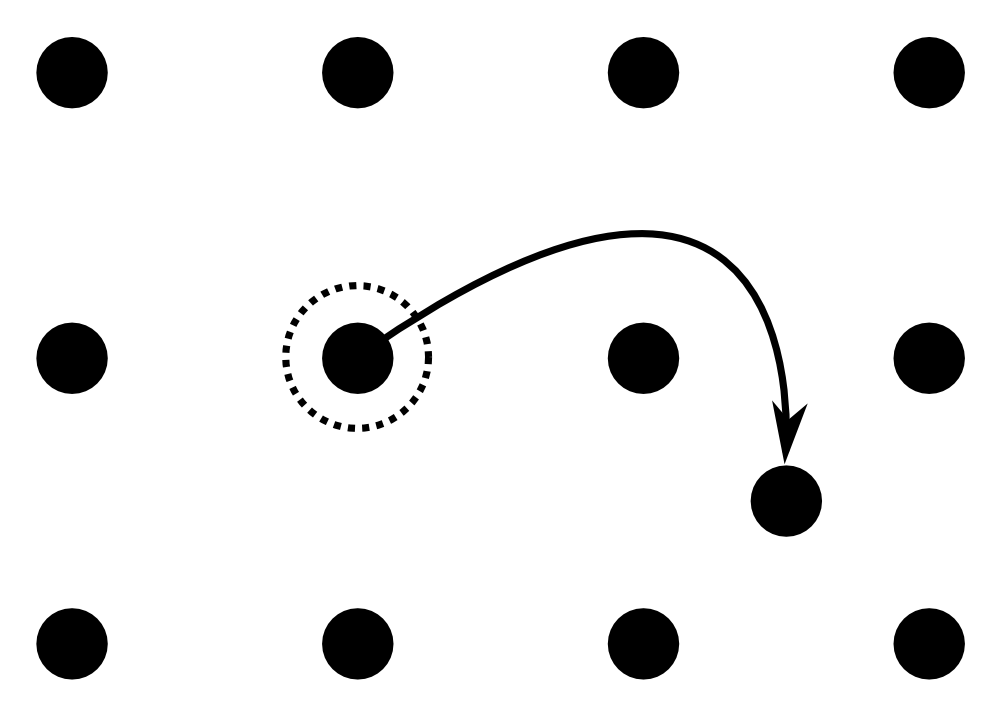
\includegraphics[width=0.75\textwidth]{kap04_01.png}

\underline{C Fremdatome}

\(C'\) interstitielle F.A.
\(C''\) substitutionelle F.A.

Si-Dotierung: z.B: \(S_i^{4+}\rightarrow Ga^{3+}\), \(S_i^{4+}\rightarrow P^{5+}\)

\underline{Experimentelle Methoden}:

\begin{itemize}
\item ESP = Elektronenspinresonanz + Optik
\item NMR = Kernspinresonanz + Optik
\end{itemize}


\section{Ausgdehnte Deffekte: 1D - Defekte}

Versetzungen (engl. dislocations) sind für Mechanische Eigenschaften
von Festkörpern verantwortlich. 


%\includegraphics[width=0.75\textwidth]{08_02.png}
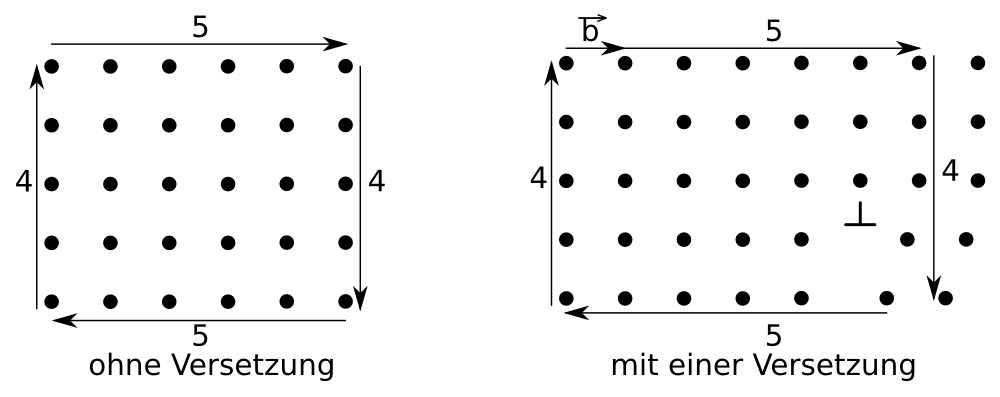
\includegraphics[width=0.75\textwidth]{kap04_02.png}

\(\vec b\) - Burgers-Vektor
\(\perp\) - Stufenversetzung

zwei Grundtypen von Versetzungen

%\includegraphics[width=0.75\textwidth]{08_03.png}
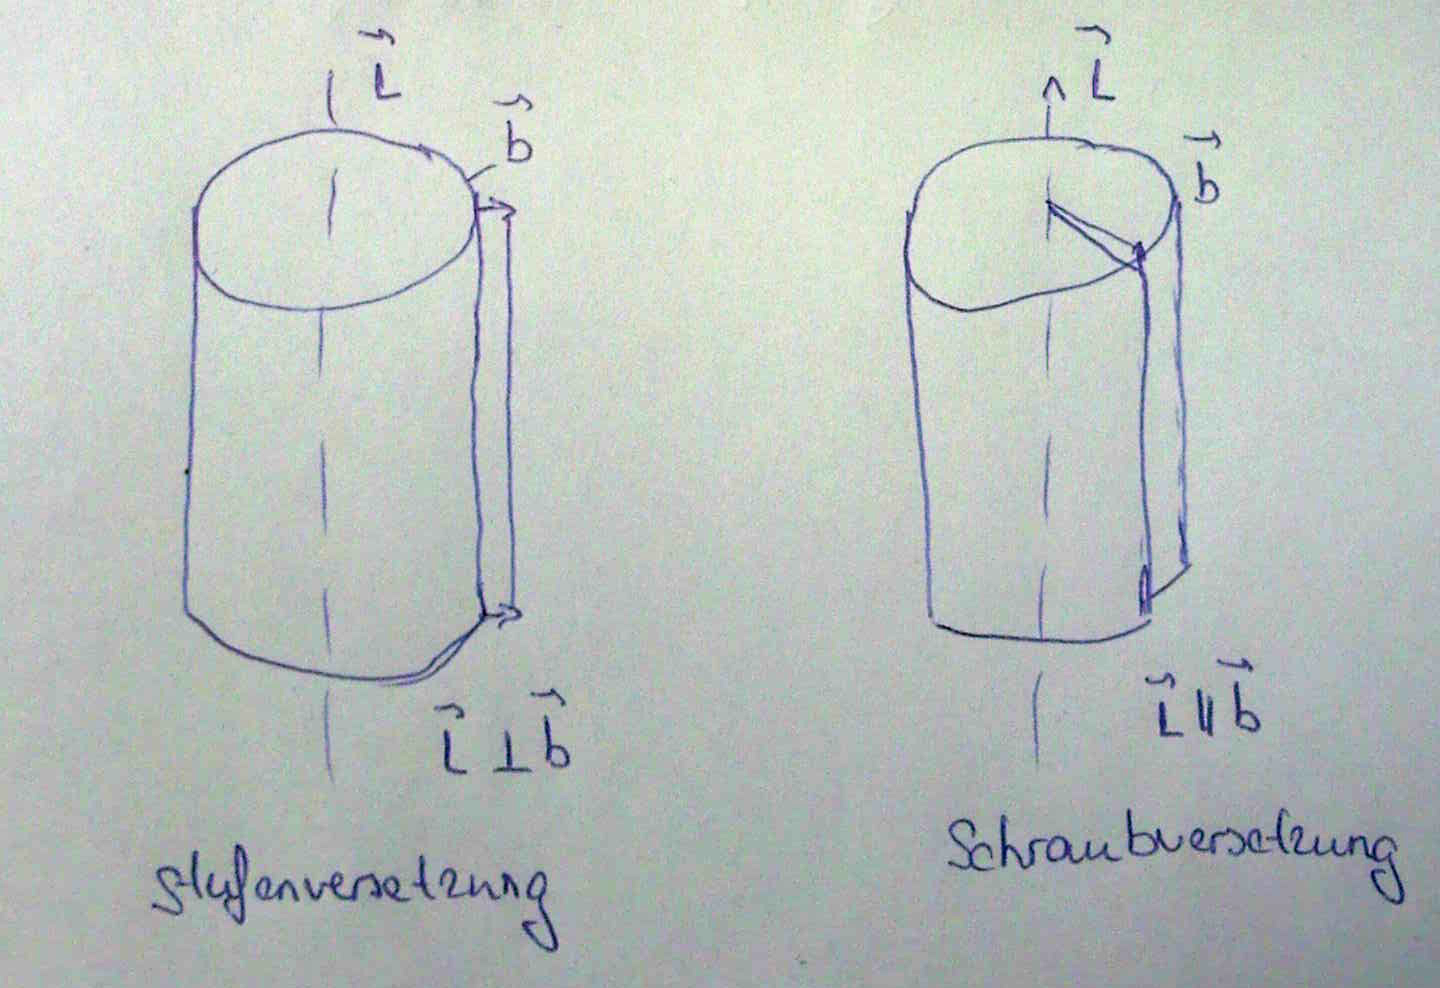
\includegraphics[width=0.75\textwidth]{kap04_03.png}

Versetzungsknoten


%\includegraphics[width=0.75\textwidth]{08_04.png}
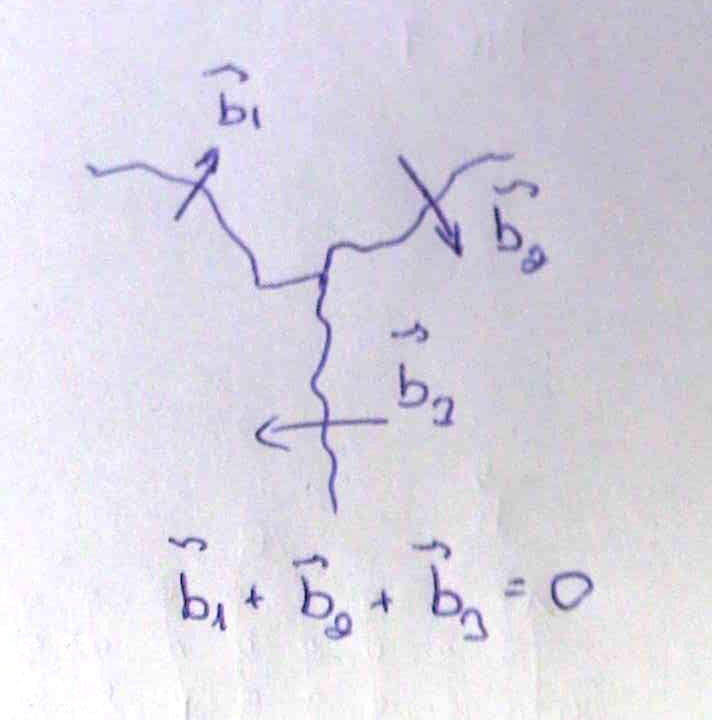
\includegraphics[width=0.75\textwidth]{kap04_04.png}

\(\vec b_1+\vec b_2+\vec b_3=0\) (ähnlich zu Kirchof). 

\(\top \bot\) - Dipol

\(\top \bot\top \bot \top \bot \top\)- Multipols

Versetzungen: a) v. Oberfläche b) Versetzungsenergie

Experimentelle Beobachtung durch chemisches Ätzen von
Probenoberflächen. (Beobachtung mit Rasterelektronenmikroskop SEM
1944).

Kristallwachstum (Whiskers) Plastische Deformationen
\[ \vec F = (\vec \sigma\cdot \vec b) \times \vec L \]

\(\vec F\)-Versetzungstensor

\section{Einkristal: Mechanische Festigkeit}

%\includegraphics[width=0.75\textwidth]{08_05.png}
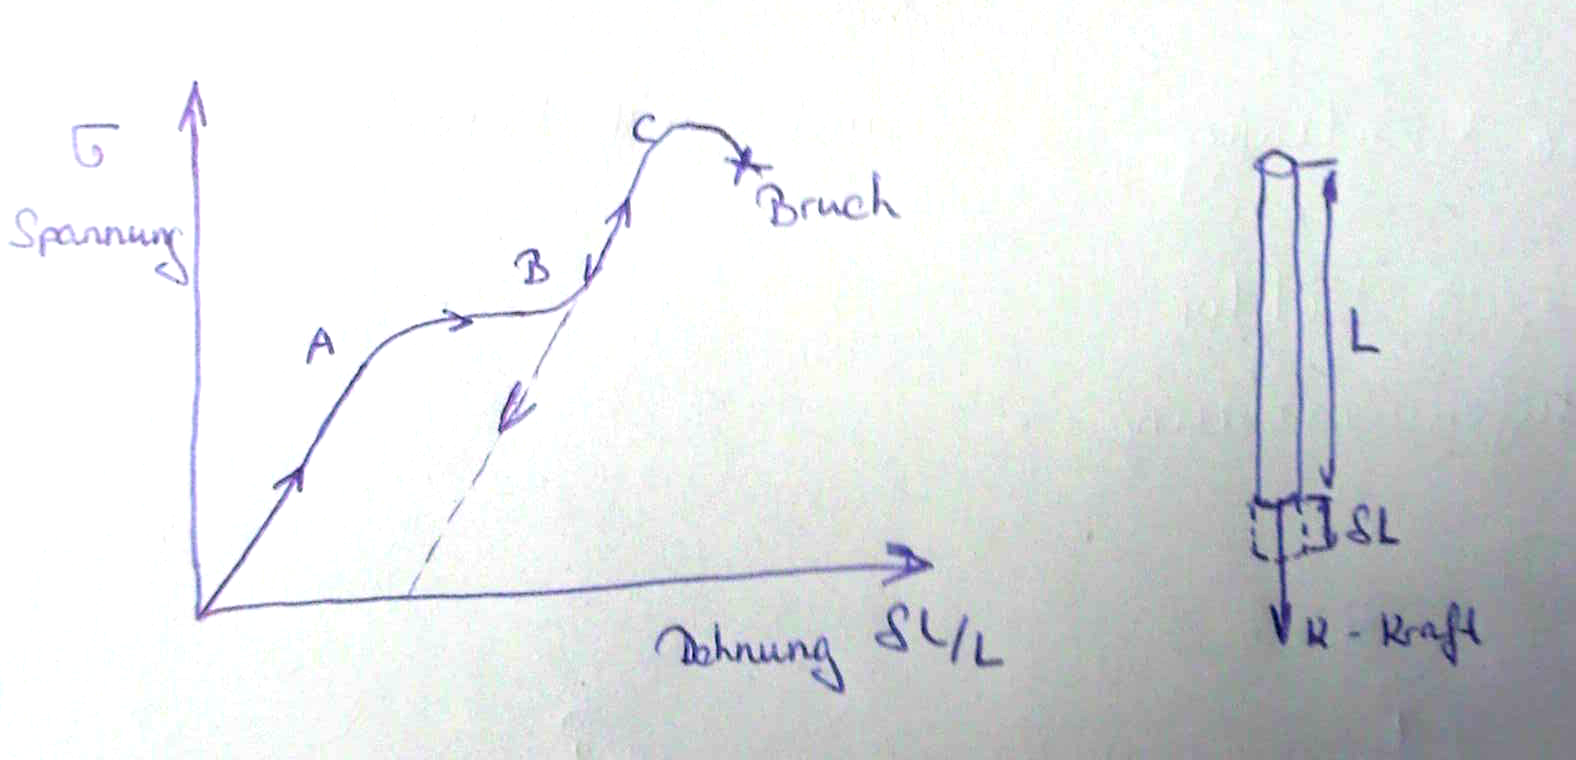
\includegraphics[width=0.75\textwidth]{kap04_05.png}

\[ \sigma = \underbrace{E}_{\text{Elastizitätsmodul}} \frac {\delta L} L \]

Erst ist die Spannung proportional zur Dehnung (Hooksche Gesetzt). Der
Bereich zwischen A und B wird Dehnung größer ohne größer werden von
Spannung. Hier finden Versetzungen statt. 

A-B Plastische Deformation
B-C Verfestigung

Einkristalle \(\approx 10^2-10^5\) Versetzungen\(/cm^2\)
Kalt verformte Metalle \(\approx 10^{12}\) Versetzungen\(/cm^2\)


\section{Plastische Deformationen}


%\includegraphics[width=0.75\textwidth]{09_01.png}
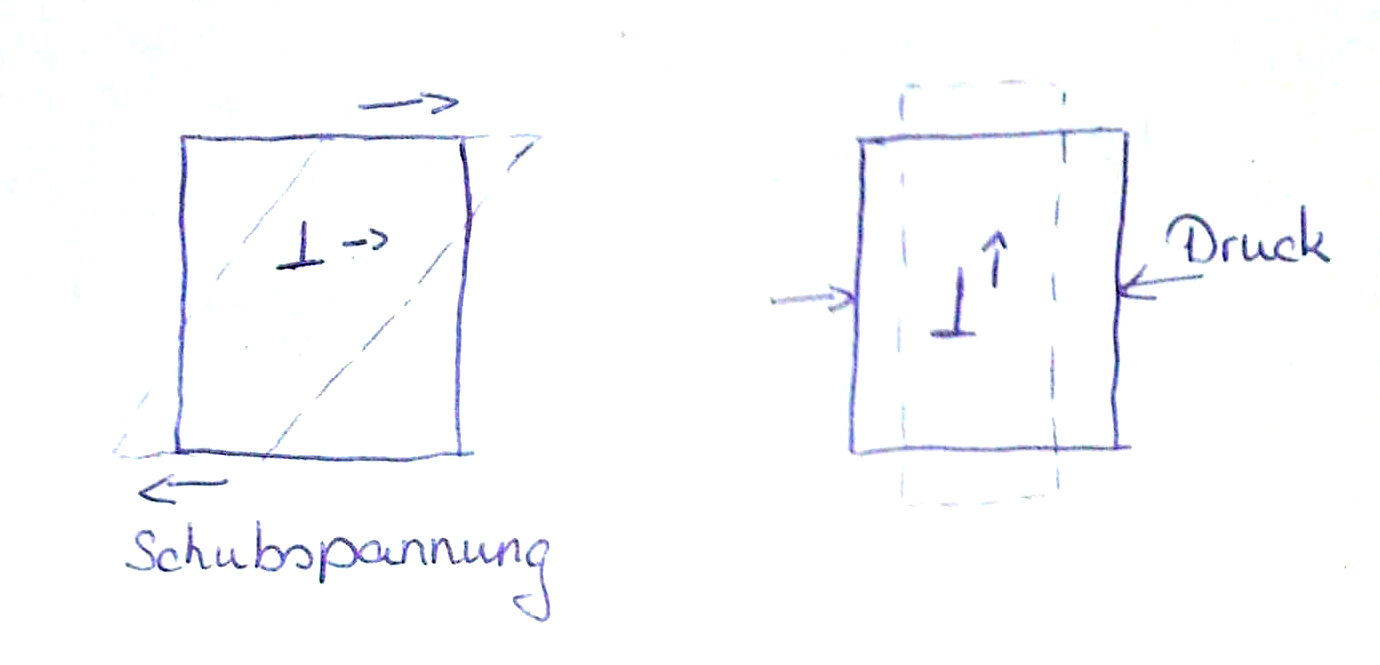
\includegraphics[width=0.75\textwidth]{kap04_06.png}

\[ \vec F (\sigma\cdot \vec b) \times \vec L \]

Whiskers (engl.) =  Vibrisse (lange Stäbchen mit Versetzung)

\underline{2D Defekte}: Korngrenzen = Bereiche zu Kristallite (Polykristalle)

Kleinwinkelkorngrenzen 

%\includegraphics[width=0.75\textwidth]{09_02.png}
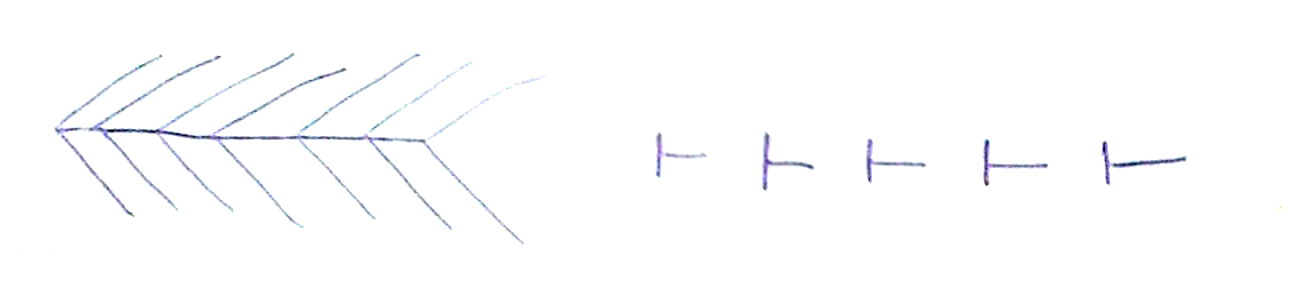
\includegraphics[width=0.75\textwidth]{kap04_07.png}

Stapelfehler: fcc und hcp   A B C A B C|A B|A B|A B C...

\section{Amorphe Materialien}

Paarvertelungfunktion eine Atomsorte

\[ g(\vec r_1, \vec r_2) = \frac 1 {n^2_0} \langle n(\vec r_1)\cdot
n(\vec r_2) \rangle \]
%\includegraphics[width=0.75\textwidth]{09_03.png}
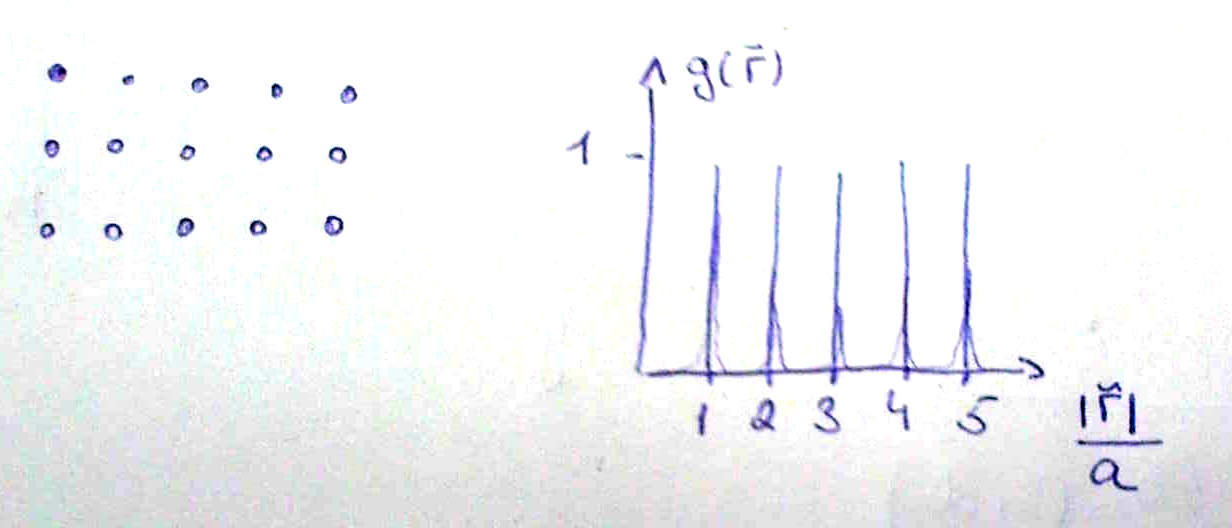
\includegraphics[width=0.75\textwidth]{kap04_08.png}

Amorphe Festkörper
%\includegraphics[width=0.75\textwidth]{09_04.png} 
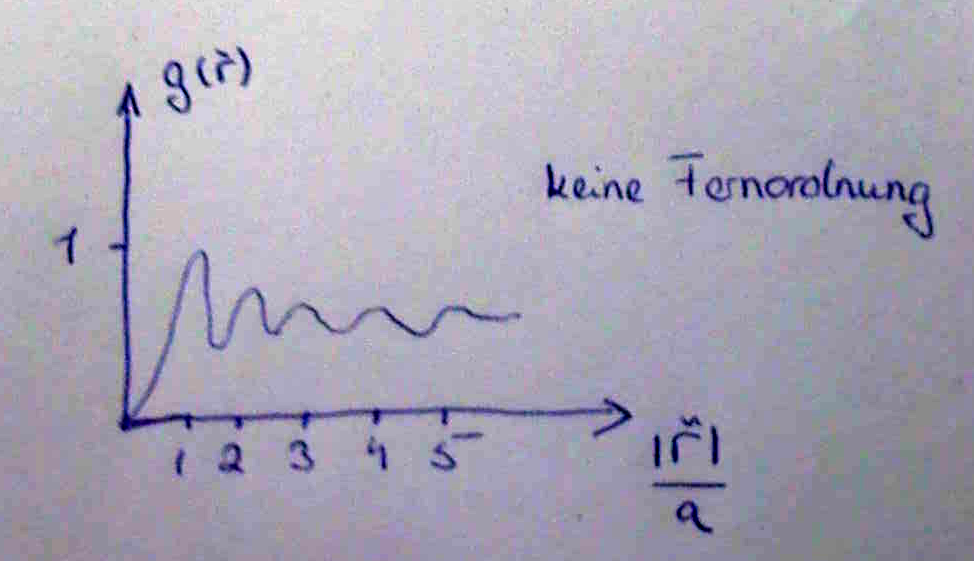
\includegraphics[width=0.75\textwidth]{kap04_09.png} 

keine Fernordnung (metabstabil)

%\includegraphics[width=0.75\textwidth]{09_05.png}
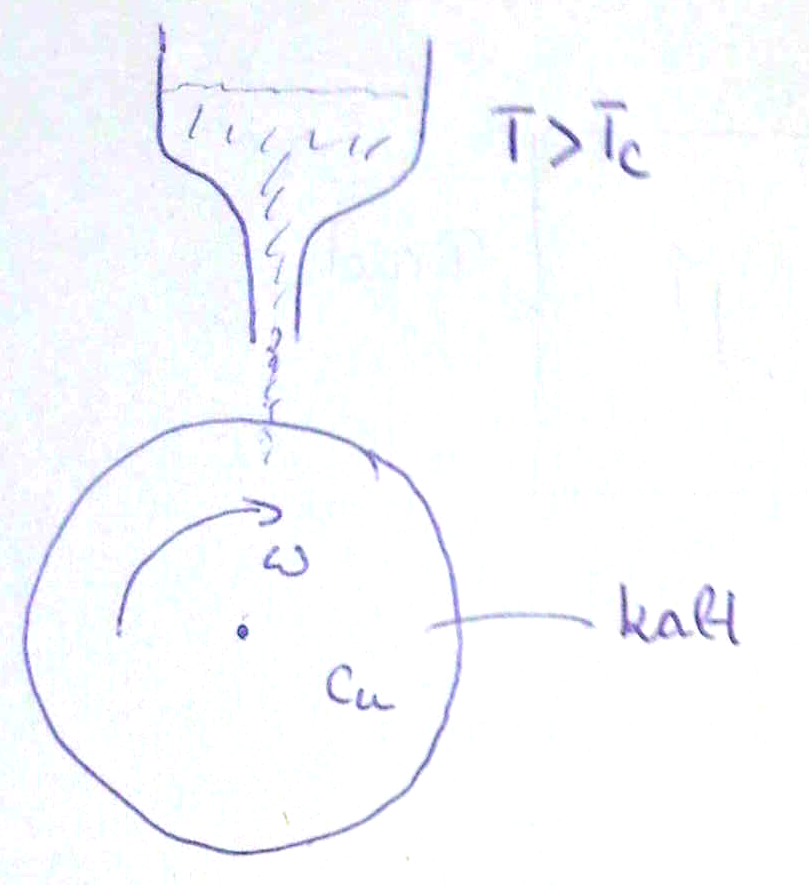
\includegraphics[width=0.75\textwidth]{kap04_10.png}

Festplatten sind von amorphen magnetischen Material gemacht. In
Flüssiger form wird das material auf eine rotierende disk getropft und
erstarrt dort.

Anwendungen:
\begin{itemize}
\item Festplatten
\item \(\alpha\)-Si (Solarzellen)
\end{itemize}

